
\section{Example: Validation of PISM as a flow model for the Ross Ice Shelf in Antarctica}\label{sec:ross} \index{PISM! diagnostic Ross ice shelf setup}\index{Ice Sheets!Antarctic ice sheet!Ross ice shelf} \index{PISM!validation of ice shelf model} \index{Ross ice shelf}
\optsection{Ross}

The term ``validation'' describes the comparison of model output with physical observations in cases where those physical observations are believed to be sufficiently complete and of sufficient quality so that the performance of the numerical model can be assessed \cite{Roache,Wesseling}.  Roughly speaking, validation can happen when the observations or data are better than the model, so the comparison measures the quality of the numerical model and not merely errors in, or incompleteness of, the data.

As part of the first EISMINT series of intercomparisons, MacAyeal and others \cite{MacAyealetal} validated several ice shelf numerical models using the Ross ice shelf as an example (i.e.~``EISMINT-Ross'').  The models were compared to velocity data from RIGGS Survey \cite{RIGGS2,RIGGS1}, acquired in the period 1973--1978 and measured at a few hundred locations in a grid across the shelf.  Substantial developments followed EISMINT-Ross, including inverse modeling to recover depth-averaged viscosity \cite{RommelaereMacAyeal} and parameter-sensitivity studies \cite{HumbertGreveHutter}.  Previous PISM versions included a specialized executable \texttt{pross} that set up the EISMINT-Ross flow model and performed the diagnostic computation.

Increased availability of data sets for ice sheet modeling, including the public ALBMAP v1 \cite{LeBrocqetal2010} data set for ice sheet modeling, and the MEaSUREs InSAR-Based Antarctica Velocity Map \cite{Rignotetal2011} in particular, make it possible to create a similar setup using more complete, recent, and higher-resolution data.

The scripts in this section are found in the directory \texttt{examples/ross/}.  In summary, the script \texttt{preprocess.py} will download data and build a NetCDF input file and the script \texttt{run.sh} runs PISM.


\subsubsection*{Grabbing the data}

Our setup uses geometry and surface boundary condition data from the ALBMAP and surface velocity from MEaSUREs.  (See \texttt{preprocess.py} for URLs of these data.)  We use NetCDF Operators to cut out the relevant portion of the grid and CDO to conservatively-interpolate high-resolution (500 m) velocity data onto the coarser (5 km) geometry grid used in ALBMAP.  The script \texttt{nc2cdo.py}, included in the PISM distribution in directory \texttt{util/}, prepares the NetCDF file for the application of CDO, which requires complete projection information.  Run

\begin{verbatim}
$ python preprocess.py
\end{verbatim}%$

The NetCDF file \texttt{Ross_combined.nc} produced by \texttt{preprocess.py} contains ice thickness, bed elevations, surface temperature, net accumulation, as well as latitude and longitude values.  All of these are typical of ice sheet modeling data, both in evolution and diagnostic runs.

The file also has variables \texttt{u_ssa_bc} and \texttt{v_ssa_bc} for the boundary values used in the (diagnostic) computation of velocity.  They are used at all grounded locations and ice shelf cells that are immediate neighbors of grounded ice.  The variable \texttt{bcflag} specifies these locations.


\subsubsection*{Diagnostic computation of ice shelf velocity}
A diagnostic Ross ice shelf velocity computation from these data initializes from \texttt{Ross_combined.nc} and does a zero-year run:

\begin{verbatim}
$ mpiexec -n 2 pismr -boot_file Ross_combined.nc \
          -Mx 211 -My 211 -Mz 21 -Lz 3000 -z_spacing equal \
          -no_sia -no_energy -ssa_floating_only -pik \
          -ssa_dirichlet_bc -y 0 -o out_211.nc -o_order zyx
\end{verbatim}%$
The computational grid here is the ``native'' $5$ km data grid used in ALBMAP.  The maximum thickness of the ice is $2766$ m so we choose a height for the computational box large enough to contain the ice (i.e.~``\texttt{-Lz 3000}'').  There is no need to type in the above command; just do

\begin{verbatim}
$ ./run.sh 2
\end{verbatim}%$

\noindent Several command-line options require explanation:
\begin{itemize}
\item \texttt{-no_sia} turns off the SIA stress balance computation, since our
  goal is to model the ice shelf. It also side-steps a technical issue: PISM
  uses periodic boundary conditions at domain boundaries and most fields in
  this setup are not periodic. Turning off SIA avoids operations such as
  differencing surface elevation across the domain edges.  For a more complete
  solution to this technical issue see section \ref{sec:jako} on a regional model using
  option \verb|-no_model_strip| and executable \verb|pismo|.
\item \texttt{-ssa_dirichlet_bc} reads fields \texttt{u_ssa_bc}, \texttt{v_ssa_bc}, \texttt{bcflag}, and \texttt{thk} from an input file and uses them to prescribe Dirichlet boundary conditions for the SSA velocity (\texttt{u_ssa_bc} and \texttt{v_ssa_bc} are components of the SSA B.C., \texttt{bcflag} is $1$ at B.C. locations and $0$ elsewhere) and \texttt{thk} at $\mathtt{bcflag} = 1$ locations is used as the Dirichlet B.C. condition for the ice thickness. The latter (together with Dirichlet B.C. for the SSA velocity) can be thought of as prescribing ``SSA ice flux'' at given locations in an \emph{evolution} run.
\item \texttt{-ssa_floating_only} uses the SSA stress balance model for the floating ice \emph{only}. In this setup it is actually equivalent to \texttt{-ssa_sliding}, because SSA velocities at grounded locations are prescribed.
\item \texttt{-pik} enables PIK improvements (see section \ref{sec:pism-pik}). The most important one here is the calving front stress boundary condition (CFBC), option \verb|-cfbc|.
\item \texttt{-y 0} makes PISM stop after the first one-model-second-long ``preliminary'' time-step.  The model state is reset after this time-step, making it equivalent to a ``diagnostic'' run.
\end{itemize}

The script \texttt{run.sh} allows changing grid resolution and using the SSA flow law enhancement factor as a tuning parameter.  There are many reasonable choices of tuning parameters, and using an enhancement factor acknowledges that the physical justification for tuning is uncertain.  One could instead use ice softness in an isothermal setup, or temperature in a thermomechanically-coupled setup, for example.  Even the density of the ice shelf might be used as a tuning parameter, because high accumulation rates and cold firn, and basal freeze-on of marine ice, may generate significant changes in shelf density.

The script \texttt{plot.py} takes PISM output such as \texttt{out_211.nc} to produce Figure \ref{fig:rosspython}.  The run shown in the figure used an enhancement factor of $0.6$.  The thin black line outlines the floating shelf, which is the actual modeling domain here.  To generate your own, do

\begin{verbatim}
$ python plot.py out_211.nc
\end{verbatim}%$

\begin{figure}[ht]
\centering
\mbox{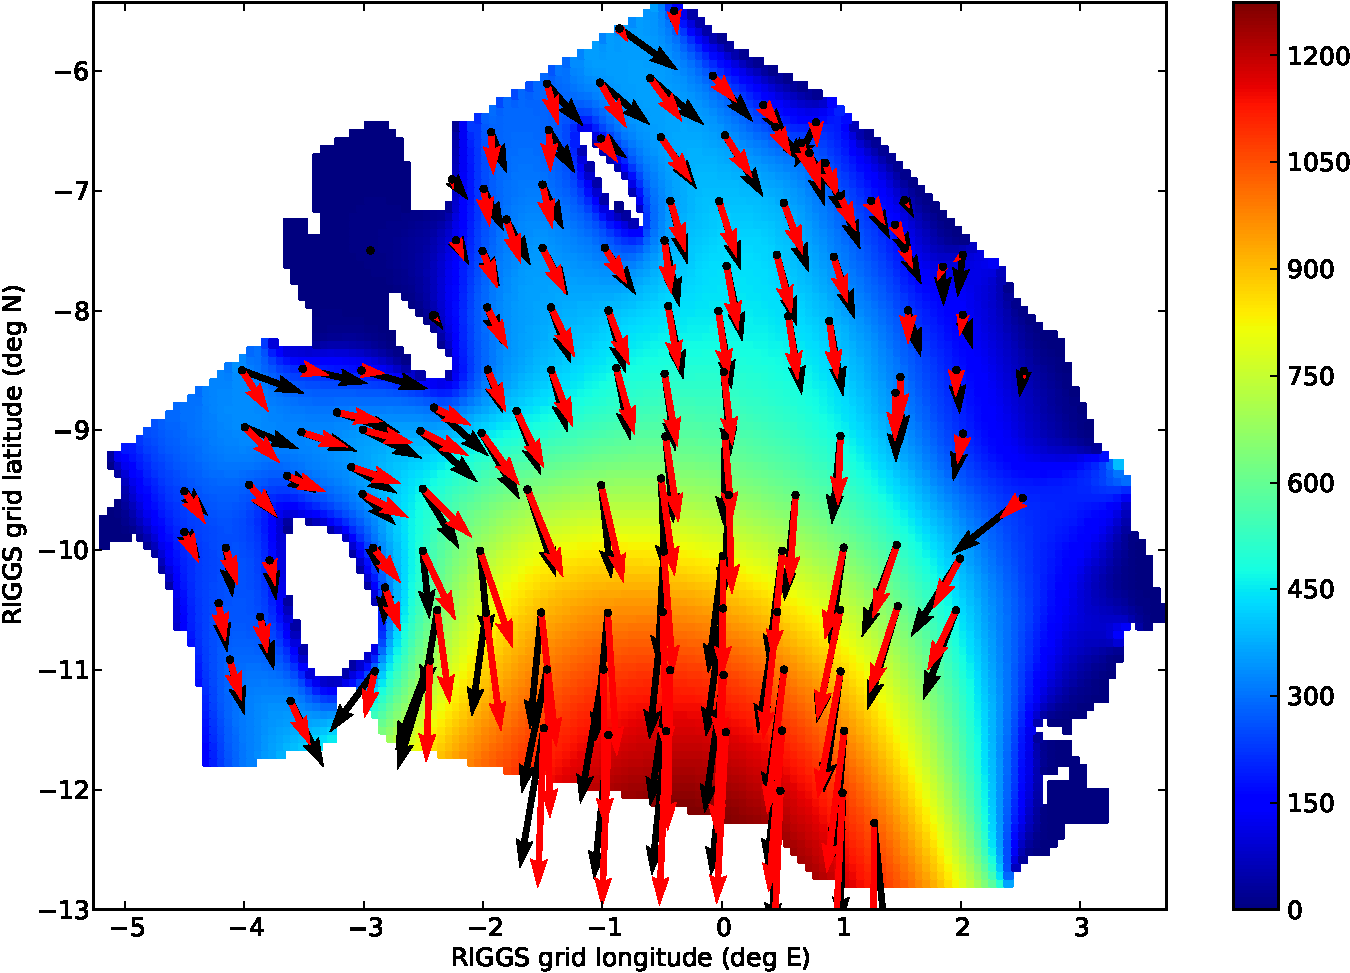
\includegraphics[width=3.3in,keepaspectratio=true]{rossquiver}\quad 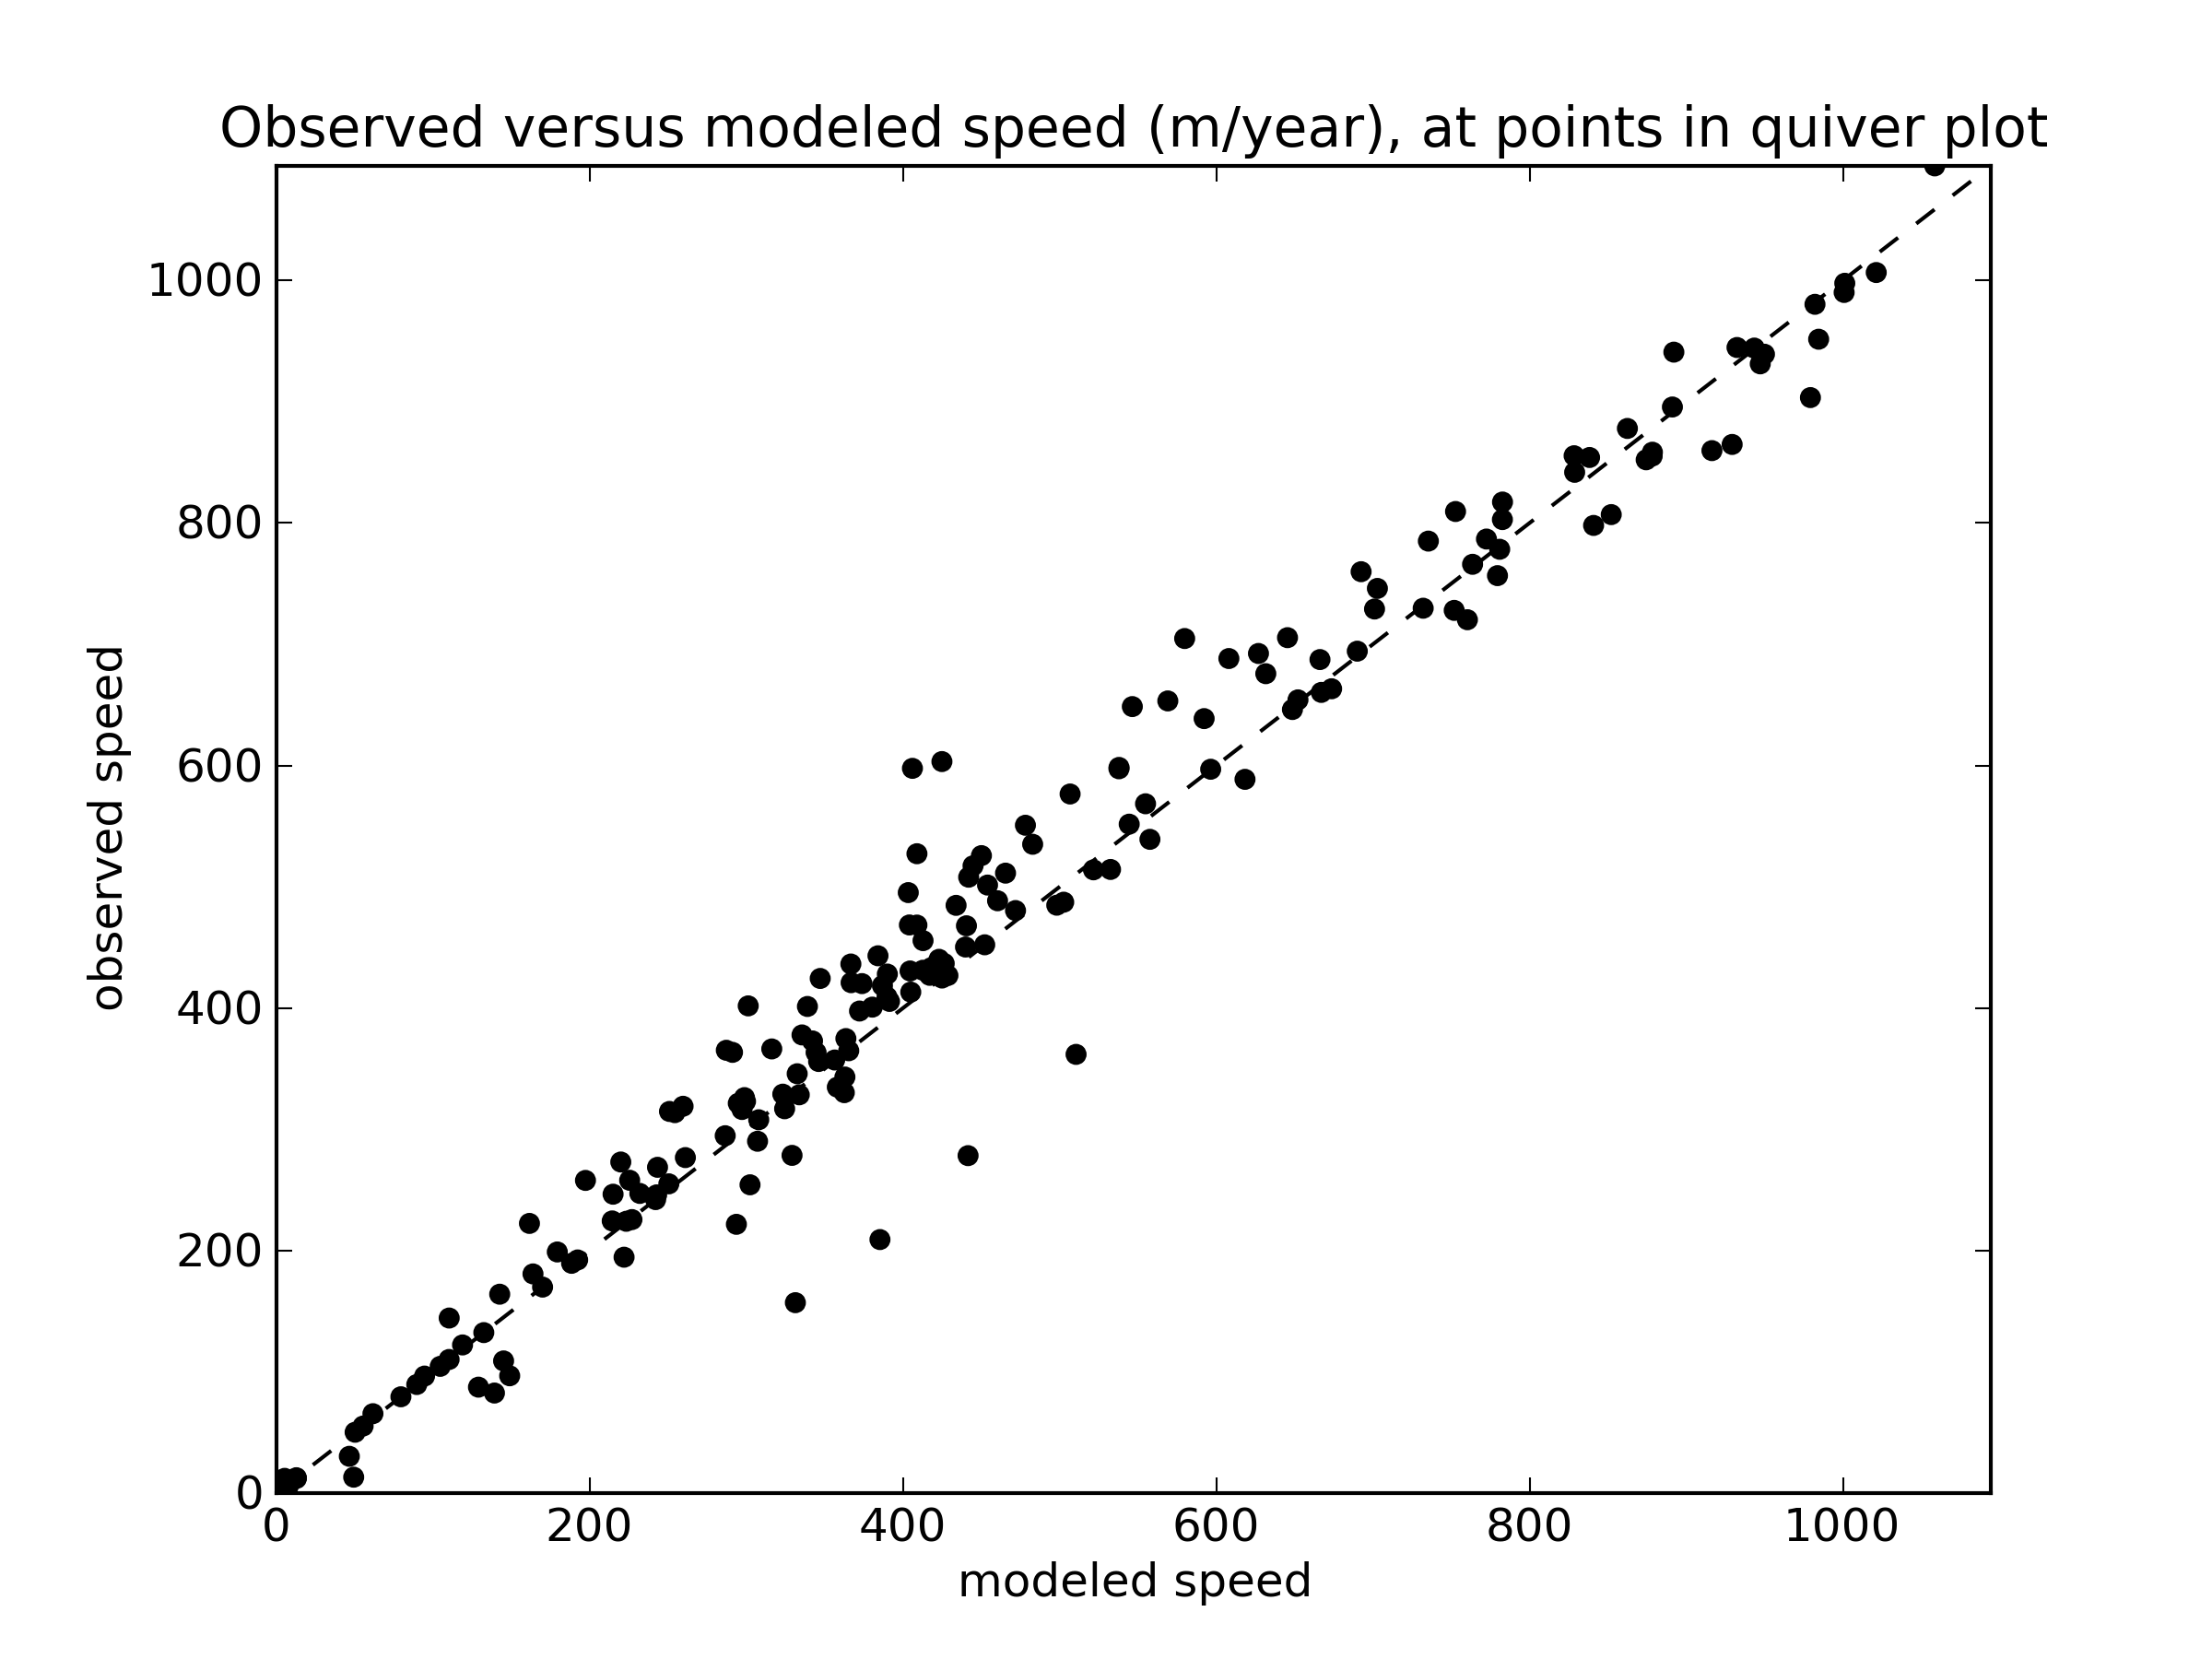
\includegraphics[width=2.7in,keepaspectratio=true]{rossscatter}}
\caption{\protect{\emph{Left}}: Color is speed in m/a.  Arrows are observed (white) and modeled (black) velocities.  \protect{\emph{Right}}: Comparison between modeled and observed speeds at points plotted on the left.}
\label{fig:rosspython}
\end{figure}

\subsubsection*{Extending this example}

\begin{itemize}
\item \textbf{Other ice shelves.}  The SSA solution described in this section can be easily applied to other ice shelves in Antarctica, including the Filchner-Ronne Ice Shelf as in \cite{AlbrechtLevermann2012}, for example.  All you need to do is to choose a different rectangular domain (within the area covered by the whole-ice-sheet data-sets used here).  In particular you should modify the line ``\texttt{ncks -O -d x1,439,649 -d y1,250,460 ...}'' in \texttt{examples/ross/preprocess.py}.
\item \textbf{Prognostic (geometry-evolving) runs.}  One can also create an evolving geometry model of an ice shelf with constant-in-time inflow across the fixed grounding line.  See \texttt{README.md}, \texttt{preprocess_prog.py}, and \texttt{run_prog.sh} in \texttt{examples/ross/prognostic/}.  This example demonstrates the \intextoption{eigen_calving} model for a moving calving front \cite{Levermannetal2012}.
\item \textbf{Evolving fracture density.}  See \texttt{README.md}, \texttt{preprocess_frac.py}, and \texttt{run_frac.sh} in directory \texttt{examples/ross/fracture_density/}.  This example demonstrates the fracture density transport model in \cite{AlbrechtLevermann2012}.
\end{itemize}

%%% Local Variables:
%%% mode: latex
%%% TeX-master: "manual"
%%% End:
